\chapter{Enterprise Service Bus}
\label{cha:esb}
An Enterprise Service Bus (ESB) is a architectural pattern which describes a distributed computing architecture, where distributed services are connected to each other via the ESB. The ESB pattern if part of the Service Oriented Patterns (SOA)  

\section{The need for an Enterprise Service Bus}
\label{sec:esb-need-for-esb}

\section{Architecture}
\label{sec:esb-architecture}

\begin{figure}[htbp]
	\centering
	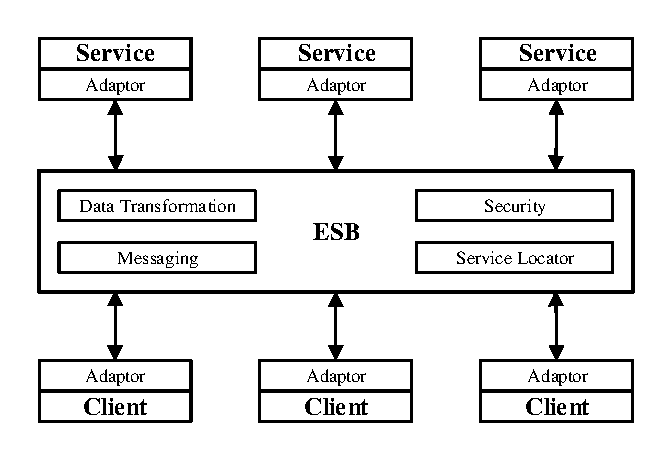
\includegraphics[scale=1]{images/esb-simple-architecture.pdf}
	\caption{Architecture of an ESB}
	\label{fig:esb-simple-architecture}
\end{figure} 

\section{JBoss Fuse Middleware}
\label{sec:esb-middleware}

\section{ESB Application}
\label{sec:esb-liwest-esb}

\subsection{Service Component Implementation}
\label{sec:esb-liwest-esb-impl}

\subsection{Service Component Logging}
\label{sec:esb-liwest-esb-logging}

\subsection{Service Component Tracing}
\label{sec:esb-liwest-esb-tracing}